% Copyright (c) 2020 Carl Martin Ludvig Sinander.

% This program is free software: you can redistribute it and/or modify
% it under the terms of the GNU General Public License as published by
% the Free Software Foundation, either version 3 of the License, or
% (at your option) any later version.

% This program is distributed in the hope that it will be useful,
% but WITHOUT ANY WARRANTY; without even the implied warranty of
% MERCHANTABILITY or FITNESS FOR A PARTICULAR PURPOSE. See the
% GNU General Public License for more details.

% You should have received a copy of the GNU General Public License
% along with this program. If not, see <https://www.gnu.org/licenses/>.

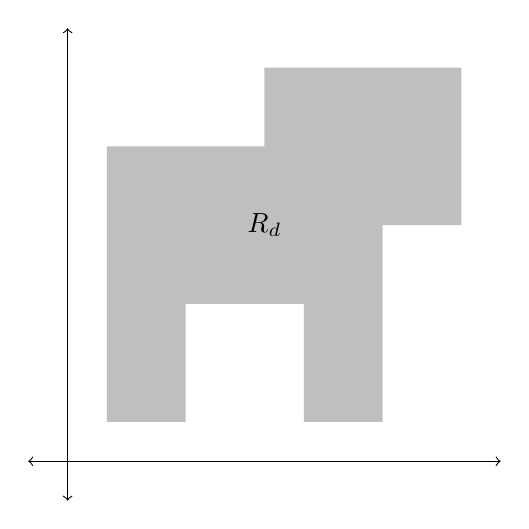
\begin{tikzpicture}[scale=1]
	
	% S'
	\fill[lightgray] (0.5,0.5) -- (1.5,0.5) -- (1.5,2) -- (3,2) -- (3,0.5) -- (4,0.5) -- (4,3) -- (5,3) -- (5,5) -- (2.5,5) -- (2.5,4) -- (0.5,4) -- (0.5,0.5);
	\draw (2.5,3) node {$R_d$};

	% axes
	\draw[<->] (-0.5,0) -- (5.5,0);
	\draw[<->] (0,-0.5) -- (0,5.5);

\end{tikzpicture}